% Miyatake-San & Xiangchong
\subsection{HSC pipline Updates}

\subsubsection{Background}

\subsubsection{Warping}



\subsection{S19A data release}
\begin{enumerate}
    \item Difference between Nexp from FDFC and that from countInput
    \item 5 vs 6 dither
\end{enumerate}

\subsubsection{FDFC region}

\subsubsection{Bright star mask}

\begin{figure*}[ht!]
\centering{
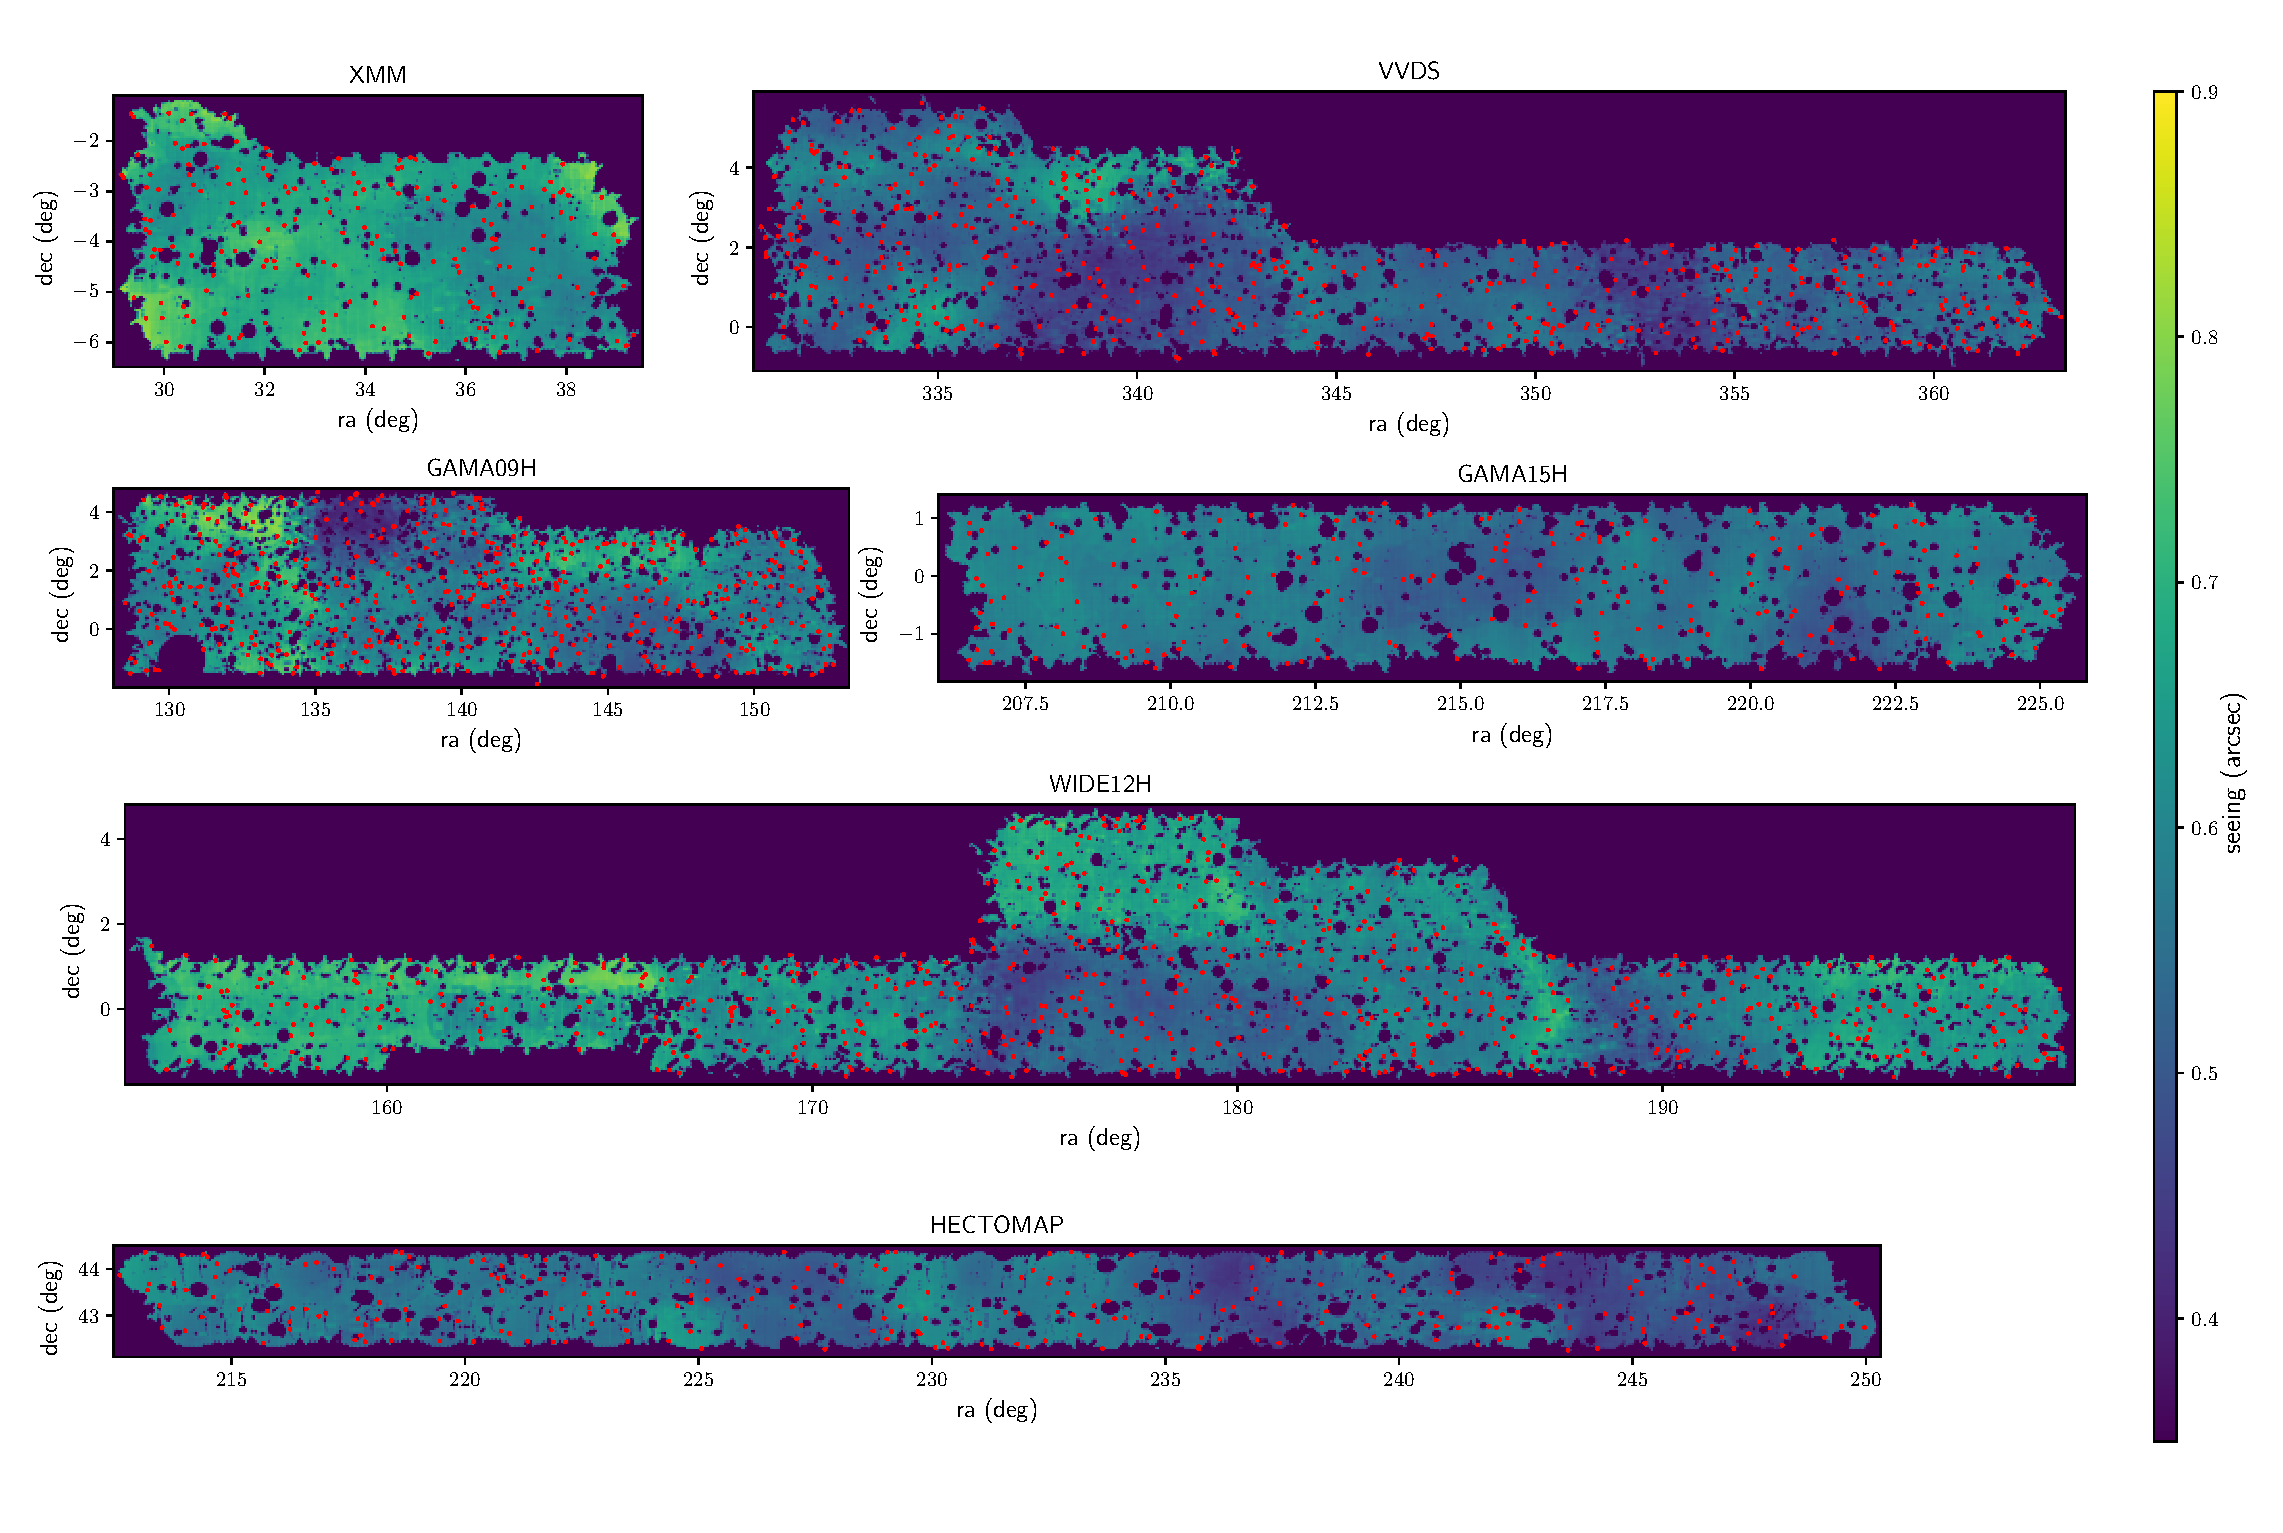
\includegraphics[width=0.9\textwidth]{fwhmMap.eps}
}
\caption{Map of the $i$-band PSF FWHM across each field. The red dots are PSFs
        used as input PSF model in the GREAT3 image simulation introduced in
        section \ref{subsec:Sim}.
    }
\end{figure*}

\begin{figure*}[ht!]
\centering{
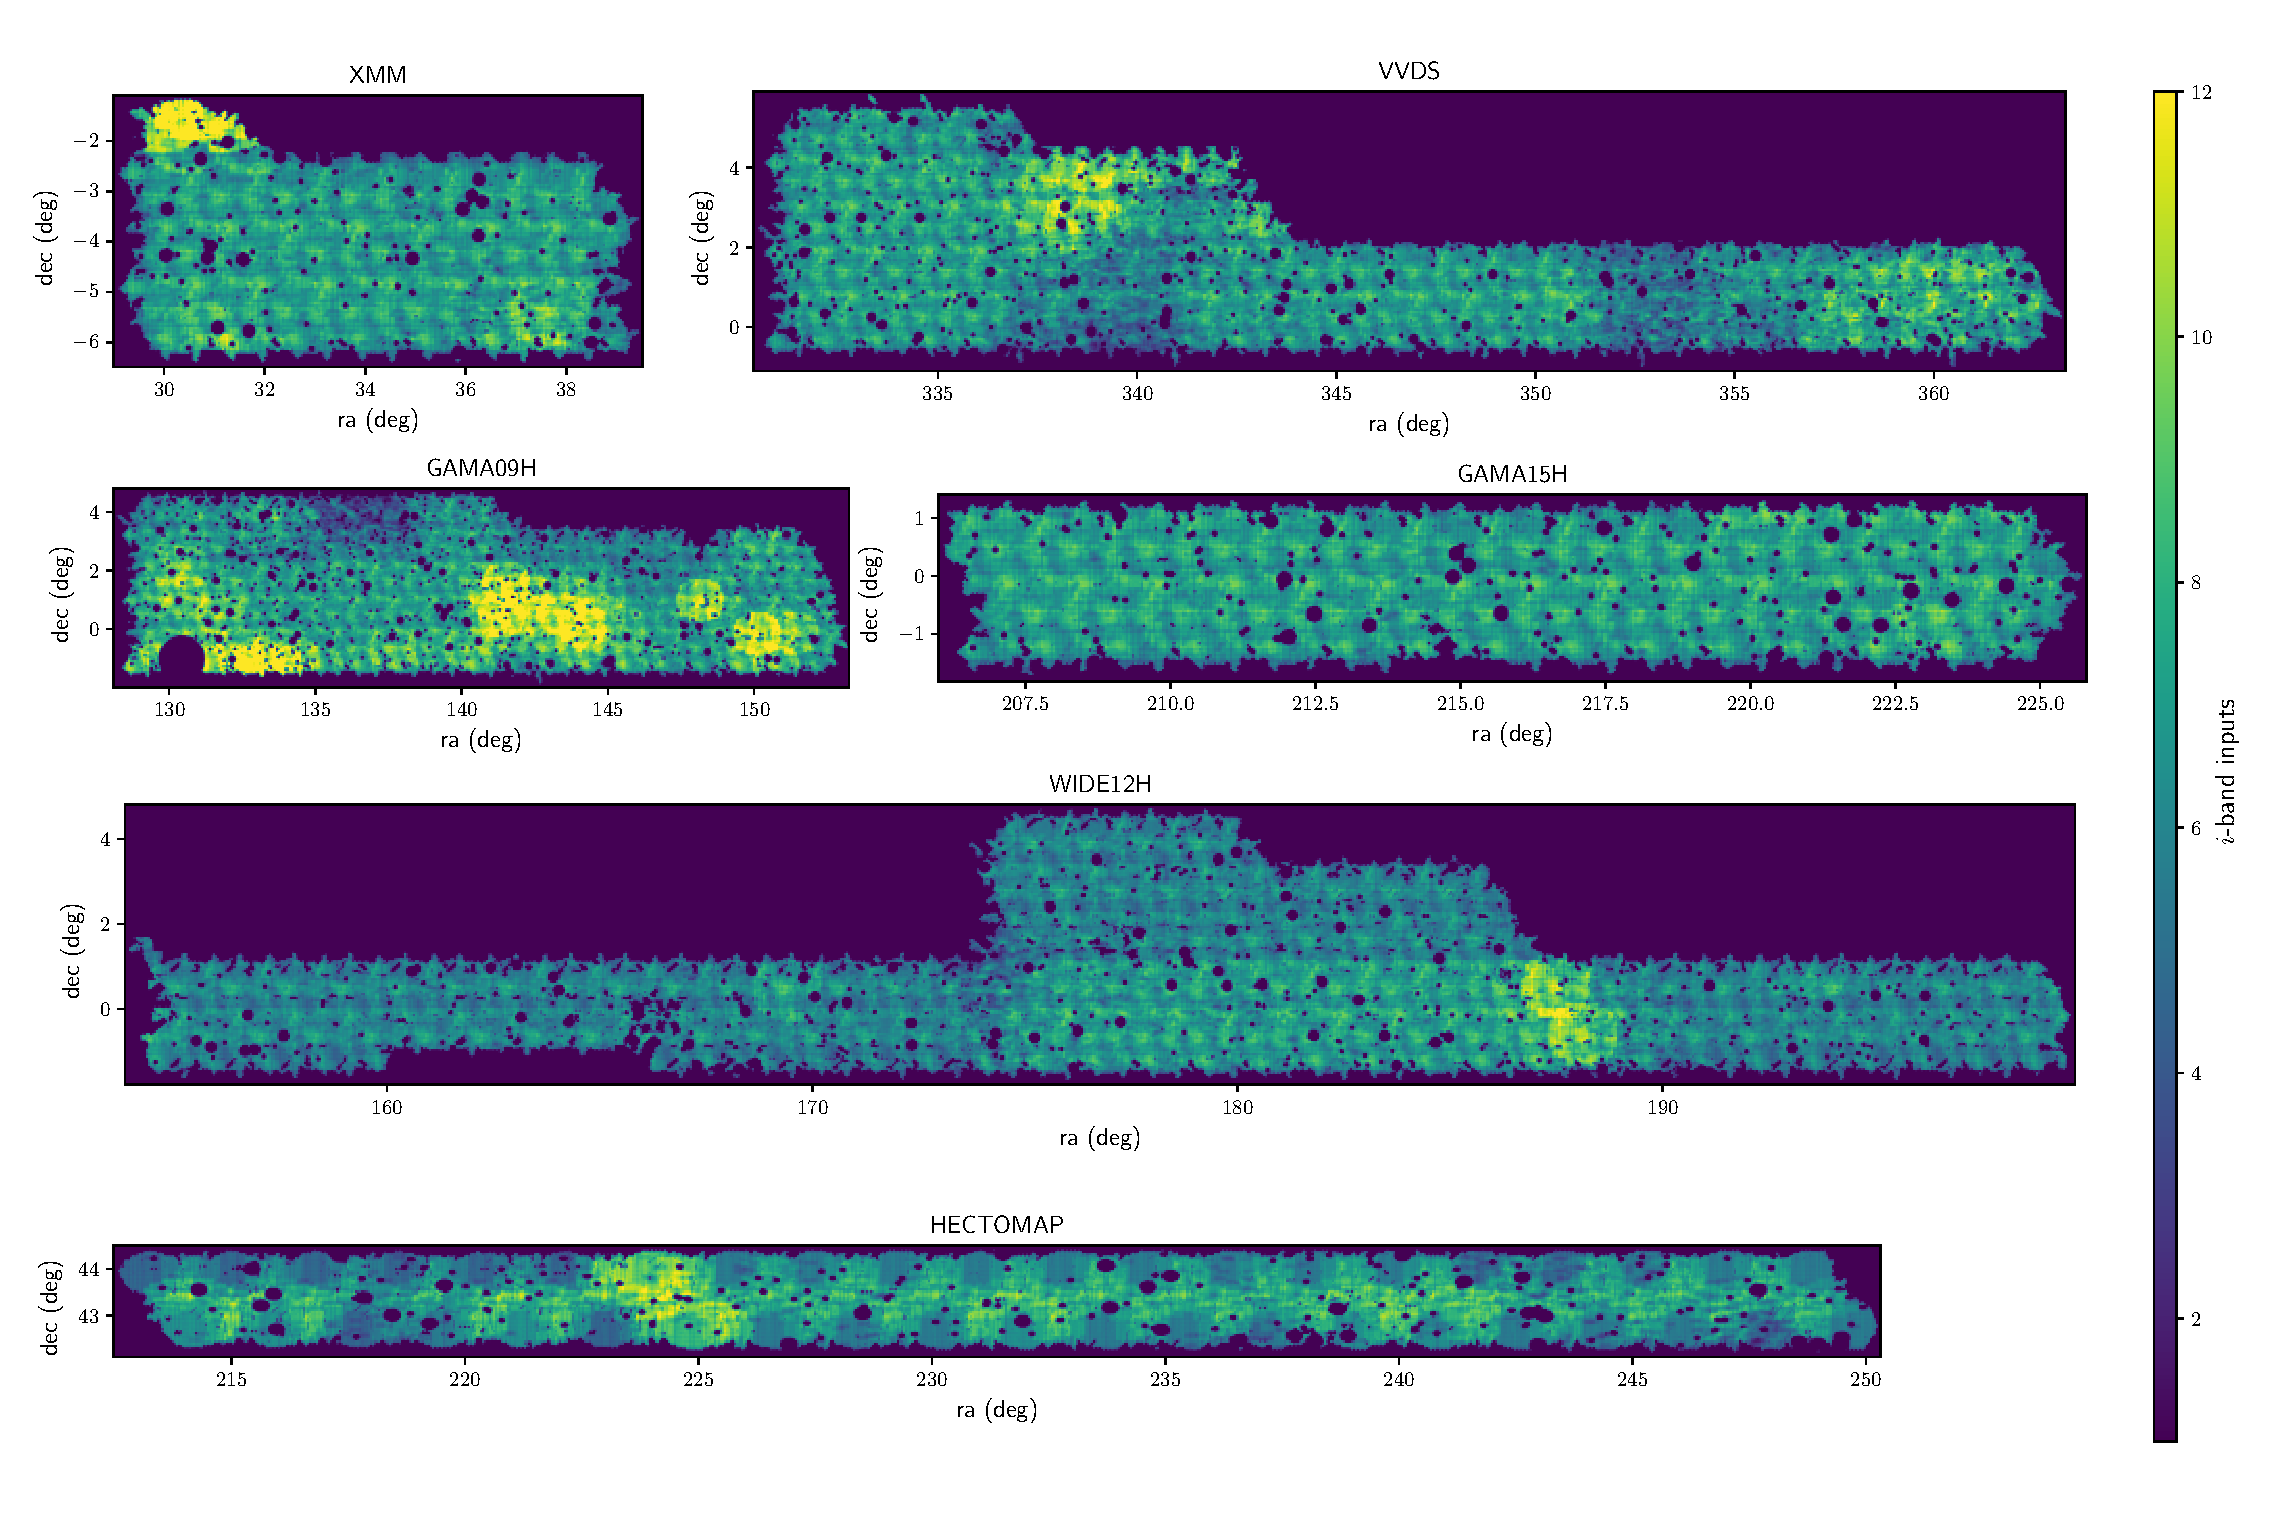
\includegraphics[width=0.9\textwidth]{icountInMap.eps}
}
\caption{
        Number of exposures contributing to the coadd in the $i$-band across
        each field.
    }
\end{figure*}
